\fancyhead[LO]{{\scriptsize 我们最幸福 · 第二十章}}%奇數頁眉的左邊
\fancyhead[RO]{\thepage}
\fancyhead[LE]{\thepage}
\fancyhead[RE]{{\scriptsize 我们最幸福 · 第二十章}}%偶數頁眉的右邊
\fancyfoot[LE,RO]{}
\fancyfoot[LO,CE]{}
\fancyfoot[CO,RE]{}
\chapter*{第二十章 · 团聚}
\addcontentsline{toc}{chapter}{\hspace{5mm}第二十章 · 团聚}
\begin{figure}[!htbp]
\centering
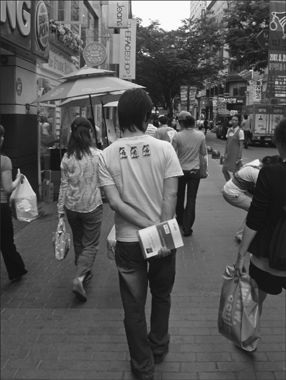
\includegraphics[width=6cm]{./Chapters/Images/20.jpg}
\caption*{2007年俊相于首尔明洞步行市场,拿着一本《1984》}
\end{figure}

曾让美兰在北朝鲜注定身处边缘生活的不洁之血在她跨过了边界之后却变成了最大的财富。家里有南韩的亲属被证明是无价的。不像其它的脱北者,要在一个陌生的世界了,独自完成脱胎换骨的重生,美兰却有着亲属张开双臂等着迎接她。\\

在南韩快节奏、高效率的现代生活之下,儒家传统仍处于支配地位。美兰的父亲,是家里的独子,是延续家族的继承人,如果他去世了,那么家族就应由他的儿女来延续。\\

当美兰一家于1998年跨过图们江来到中国后,他们要做的第一件事情就是打电话给父亲的出生地,忠清南道,西山市(Sosan)的市政厅。然而作为大规模城市化的结果,村子里的人几十年前就全部搬到城市里去了。在建了水库后,这个村子的所在地大部分被水淹没,村子自身也早就消失了。但是按朝鲜习俗,家乡就是自己父亲出生地,而不论是不是还有人生活在那里。市政办公室仍然保留有泰宇两个妹妹的地址,她们都还健在,住在首尔附近,而且市政厅也主动提议会将信件转送给她们。于是美兰23岁的弟弟,虽然是家里最小的,但是作为唯一的男性,由他提笔起草此信。他用很正式的用语写道:我作为你们哥哥唯一的儿子给你们写信。我希望通知你们,我父亲于去年在北朝鲜咸镜北道镜城县去世。他同时在信里写明了他们在延吉的地址和电话号码,延吉是他们当时所在的一个靠近边境的小城。\\

几周之后,他们接到了个电话,电话是其中一个妹妹打来的。她将信将疑的。几乎半个世纪过去了,没有电话,信件,甚至传言说她们的哥哥在战争中幸存了下来。在1961年,战争结束后8年,南韩国防部将他登记为在1953年的行动中战死。就家庭而言,他死在21岁上,没有子嗣。他的名字也被刻在国家公墓阵亡者名录上。妹妹们怎么才能知道,这不是个恶作剧,或者一个粗鄙的把戏,目的就是想从她们那里骗点钱呢?电话是美兰的姐姐接的,她告诉了姑姑们,自己所知道的事情。一些家里曾经的轶事,生日和小名。南韩的亲戚建议来个DNA测试。美兰和兄弟姐妹们都同意。\\

两个星期后,一家人团聚了。两个姑姑由家人陪同,都飞来中国,一行10人。当他们一见面,他们都目不转睛的相互盯着,意识到DNA测试完全是多余的。\\

“我们就这样一直盯着。我们惊叹的嘴都咧到了后脑勺,我们手的形状,我们说话、走路的方式是如此相像。”美兰说。\\

“我父亲的妹妹认为她们家的香火完全断了,因为我父亲是独子。”美兰的弟弟回忆道。“当父亲的妹妹来到中国,我看见她们时,我的身子一震。她们是女人,但是和我父亲长的一模一样。”\\

现在无法回头了。美兰的母亲想回清津,想和留在家的两个女儿和她的孙子、孙女们在一起,但是她们害怕北朝鲜当局会发现她们在中国的时候曾同敌国的亲属联系──这就足够杀头的了。除了南韩,她们无处可去。\\

他们的姑姑去了沈阳的南韩领事馆,询问如果将北韩的亲属带去首尔──对南韩战俘的遗孀和子女目前他们至少能做什么──然而领事馆对这些问题也是吱吱呜呜,说不出个所以然。金大中,他于后来荣获诺贝尔和平奖,于1998年2月正式成为南韩总统,当时发起了“阳光政策”以缓和与北朝鲜的关系。而且,南韩与中国的关系也很敏感。那些官员害怕接纳美兰一家会导致严重的外交后果。\\

幸运的是,亲戚们自己想办法解决了问题。姑姑们经营着一个小酒店,她们有个儿子在首尔郊外有间浴室。他在中国与南韩之间来来回回,帮北朝鲜的亲戚们弄了些伪造的非常真实的护照。他还把和美兰差不多大年纪的一个表妹的护照给了她。表妹的照片被拿掉,换上了美兰的。一个姑姑不巧“丢了”自己的护照,这样那本护照就可以给美兰的妈妈。实际上,这些都是非法的活动,后来表妹还因伪造护照被关了一个月,但是这起了作用。美兰、姐姐、弟弟和妈妈都于1999年1月都安全的抵达了南韩。\\

由于有家庭接纳她,美兰没有被太多的认为是外来的人,一个曾经在其它地方度过了人生头二十五年的南韩人。对北朝鲜人来说,她出类拔萃,但是对南韩人来说就不会了。她身高160公分,对北朝鲜人来说属于身材高挑的,对南韩人来说也就过得去吧。她还有着让俊相在剧院外迈不开步子的高高的颧骨和直直的罗马式的鼻梁。姣好的面容、家庭的系带、镇定和天资聪颖还是使她与众不同。她很快被一个教育学位项目接纳。她口齿清晰,能以很简洁明了的方式叙述一个事情,因而她经常被邀请去做关于北朝鲜教育系统的演讲或访谈。\\

就在快要30岁的时候,她被介绍给一个身材高大的年轻男子,他憨厚的笑容和圆圆的眼镜传递着热情。他有份不错的工作,作为文职人员供职于军队。在双方家庭的赞许下,他们结婚了。在2004年末,她生下了一个儿子。他们以传统的朝鲜方式庆祝着他们的第一个孩子,宴请了将近100多位亲戚朋友。餐厅的房顶以蓝白气球装饰。美兰,她丈夫,还有小婴儿都穿着华美的韩服(Hanbok),一种在庆祝场合下穿的传统服饰。美兰的外套是闪亮的乳白色丝质面料、配有绣花的红丝带和黑色的领圈。她看上去容光焕发,而又端庄沉稳,一个非常优雅的女主人。她已经实现的她的朝鲜梦,事实上也是我认识的所有人的梦想──帅气的丈夫、男婴及其口袋里的大学文凭。\\

从穿着,说话方式,她已经和一个南韩人没什么区别了。她已经改掉了喉咙音口音,那种会泄露身份的北朝鲜人的发音特征。她和丈夫在水原这个卫星城买了个公寓,夫妻俩刚刚起步,他们还承担不起在首尔动辄百万美元的公寓。她住在一个楼盘里,这个楼盘就是个千篇一律的混凝土森林,除了侧面印着的楼层数字外,每一层都是一样。在小区里转转,其实也还不错。建筑都很新很干净,立面都刷着令人愉快的奶油色。阳光穿过大型落地窗,照在美兰位于二楼公寓的起居室里。公寓里明亮,宽敞,有专门给宝宝的浴室,一间桌子上配有三星计算机的书房,一个电器配备齐全的开放式的厨房。\\

当我去拜访时,她正在做午饭,而她的儿子,现在是个圆嘟嘟、蹒跚学步的小孩,正在起居室看着动画片。\\

“如果我是在北朝鲜生的他,我现在只能用米汤加点糖喂他,如果买得起的话。”她说。\\

我们谈论着她现在生活的变化。她正纠结于家庭和学位学习之间的冲突。她的婆婆希望她做个传统的朝鲜主妇。请人照看孩子很贵;她发现现在很难完成功课。她现在也去做有氧运动以期进行产后恢复。她总会觉得皮肤很紧。显然,她身上的问题与我认识的其它在职母亲没有什么不同。\\

然而,内心里,美兰还是那个在北朝鲜身处底层社会,贫穷,不洁之血的女性后代。她曾被一种彻底的教化塑造,并且经历着背叛的痛苦;多年来,她不敢说出内心感受,那些藏在心里的出格的想法。她曾经坚定的从死人的尸体傍走过,而不曾停下脚步。她学会闷头吃自己的午餐,吞下最后一勺的玉米或米饭,而不会停下来去可怜那些她教的,快要饿死的孩子。她一直被内心的负罪感所困。负罪和羞愧在脱北者中间是很普遍的;很多人憎恨自己那些为了生存的所作所为。\\

在美兰的例子里,负罪感不仅仅是一种抽象的。直到我认识她两年后,她才告诉我,留在家里的姐姐们的遭遇。在1999年夏天的时候,大概是她们抵达南韩6个月后,国家安全警察几乎同时在家逮捕了她的两个姐姐。美兰的大姐,美熙,嫁给了一个军官的家里最漂亮的女儿,她是如此的慷慨,在饥荒时给他们食物;还有姐姐美淑,曾经有着平凡的生活;她们忠于自己的父母、丈夫、孩子也忠于金正日。她们都在半夜被带走──多么类似于美兰听说过的梦魇般的场景,除了孩子被留下给丈夫,他们被强制指示离婚。据推测,姐姐们可能被送去一个劳动营服长期的徒刑。考虑到1999年严重的食物短缺,她们很可能已经死去。\\

姐姐们的命运深深的牵动这全家,也使任何一个欢快的时候都蒙上一层阴影。即使是美兰生了个健康的宝宝,而且她的弟弟、锡柱,被澳大利亚的大学录取,家里都不能尽情欢乐。这看上去非常不公平。几年后,脱北者可以送钱回去,他们的亲人也被放回家,没有遭到报复,甚至生活的比一般北朝鲜人还要好。可能姐姐们受到特别严厉的惩罚是因为美兰家是第一批逃离的,也可能是因为他们不好的成分。美兰的母亲,一个意志坚强的女人,想方设法的度过饥荒,在抵达南韩后,也倒下了。虽然抵达时才62岁,她的身体和精力已大不如前。她请了一个巫师、一个传统的算命师,他告诉她,女儿们还活着,但是即使如此,这只让她更焦虑。\\

美兰的母亲开始信教。在清津在共产党之前的时期,她就参加教会,现在她恢复了儿时的信仰。她不断的祈祷,祈求宽恕自己背叛了女儿们。\\

由于没有成为信众,美兰没有这样的慰籍。她的负罪感影响着她的睡眠而且不时的在已经忙得不可开交而不应该浪费时间的时候闯入脑海。姐姐们付出了极大的代价才让她现在可以开着现代车。\\

她还想到了落下的男友。她对于他敦促自己去反抗出身低的命运,给她以作为女人和教师的自信。他从来没有在她面前说这个政权一个字的坏话,但是他已经教过她用自己的脑子去思考,而这最终使她保持开放及清晰的思维。\\

当我们相会时,美兰经常提及俊相。我怀疑她很享受追忆自己的初恋──而这些是不能同母亲,当然也更不能同丈夫谈及的。当她回忆俊相是怎么第一次在剧院外遇见她,或者她们如何整夜的在黑暗里行走,那些话语就滔滔不绝的喷涌而出,兴奋的就像个女学生在和朋友闲话着。\\

“你能相信吗?3年才牵手,6年才接吻?甚至都算不上是个吻,真的,就是碰了碰脸颊。”\\

我们开玩笑的说那是不求回报,或者在这个例子中是未完成的,爱情是唯一永恒的。看上去,好似她对先前自我清白的渴求更胜于对她的前男友。\\

我问她是否知道后来俊相怎么样了。\\

“我猜他现在应该结婚了。”她的声音渐渐低了下来,并且耸耸肩装作漠不关心。她并不后悔她们最终没在一起,她告诉我──她爱她的丈夫──但是她感到很遗憾离开的时候没有机会去道别。她记得在清津的最后一天,当她认为在街对面看到他,但是却因害怕泄露离开的计划而不敢走上前。\\

“对吧,他和我,我们有个特别的约定。我想总有一天我们会再重逢的。\\

我们是在2005年10月中旬的时候进行这一番的谈话,那是在她孩子生日聚会后的不久。3个星期后,美兰给我打电话,她的兴奋在听筒里是显而易见。她告诉了我个消息:\\

“他在这里!”\\

我们一周后,相约在首尔的星巴克喝杯咖啡,那里离我的办公室就几个街区。\\

按照美兰曾经描述过的他,我想象着一个高大、英俊的男人,有点英雄主义色彩。然而,眼前的却是个穿着牛仔裤,戴着眼镜,骨瘦如柴的家伙。然而,他身上也确实有不寻常之处。他的牙齿非常亮白,像个电影明星的。他平平的脸颊,和夸张的鼻孔让他看上去像个异族的鞑靼人\footnote{鞑靼是中国对北方游牧民族的统称,晚清特指满人──译者。},看着他让我想起了鲁道夫纽瑞耶夫\footnote{一个芭蕾舞大师──译者。}。当我们叫的卡布奇诺好了的时候,他跳起来去柜台把它们取了回来。他小心的移动着;动作很自然。另一方面,美兰却看上去很紧张。她穿着一件粗斜纹布的短裙,妆化的也比平常的浓。\\

当我正要说,作为来自一个从完全没有咖啡店的国家、刚刚抵埠人,很令人意外的是,他看上去对这些很轻车熟路,但是实际上俊相已经在南韩待了差不多1年了。当他得知美兰结婚了──从一个给他做聆讯的国家情报局的探员那里得知──他就决定不去打扰她,这样对两人都好。事实上,对于她的离开,他伤心至极,程度远远超出她的相像。她的叛逃引发了他对自己信心的一个巨大危机。他内心被他们彼此之间的荒诞关系煎熬着。为什么他们要相互保密?为什么他们两人内心都在渴望离开,但是却没有相互吐露?更严重的是,他觉得自己很懦弱,没有先行一步。他的自尊心受到伤害,不是因为她离他而去,而是因为她已经证明了自己是个勇敢的人。\\

“我以前认为我考虑的总是比她更远一步,但是我错了。”他承认。为了安慰他的自尊心,这个时候美兰插话。“那个时候,我对政府一直都是都怀疑及不信任的,但是他比我更了解外面的世界。”她朝他笑笑,然后让他继续他的故事。\\

在美兰离开后,他埋头于自己研究所的工作,之后他得到一份固定工作,而且有机会加入劳动党。他的父母和兄弟姐妹都欢欣鼓舞。这在北朝鲜可以说是好的不能再好的事情了。他在平壤的生活很惬意。他租住的房子很暖和,吃的也足够。但是他却不想定居在那儿。他也不与那些被认为和他很般配的大学女生约会。他也不再参加那些能增大他成为劳动党党员机会的额外讲座。每天晚上下班后,他就回到家,把窗帘拉的严严的,这样他就可以看南韩的电视节目。\\

2001年,俊相辞去了研究所的工作。他告诉他的领导和同事们,自己父母身体不好,作为家中长子,他要回家去照顾他们,这是听起来很合情合理的解释。然而他想回到清津的真实目的是,在那里他的行为所受到的监视会少些,而且那里距离中国边境也更近些。回家后,他打些零工,有时还会去他和美兰夜间步行时常去的那个疗养院工作。为了不浪费钱,他晚上绝大多数都是同父母待在家,即使那意味着要忍受父母那责怨般的沉默,辞职让他们对这个曾引以为豪的儿子大感失望。\\

即使深思熟虑,计划周详,然而,俊相事情进展的并不如美兰的那么顺利。\\

为了逃脱,俊相攒了3年的钱。他是个有条不紊的人,对自己的每一句话,每一个动作都有考虑。他谨慎的计划着每一个细节,甚至细到那个时候要穿什么──一件昂贵的、有泡泡图案的,叔叔从日本寄来的衬衣。如果在清津穿就太扎眼了,但是他想如果在中国穿,就没人认为他是个从北朝鲜来的乞丐。他把自己最好的日本裤子和背包装入塑料袋。他选择跨境的时间是6月,其时正值雨季水位很高。他选择了河水最深的一段,这样那里的守卫会松些。伴行的中间人带了些空的塑料瓶作为漂浮物。俊相和另一个逃亡者,一个40多岁的妇女,都脱的只剩内衣,虽然黑夜里伸手不见五指,但是他们都下意识的微微相互转过背去。俊相把所有的衣服扎进塑料袋保持干燥。\\

河水很快来到了他的下巴,而且水流也比预想的要来的强。水位却没过了另一个逃亡者的头;她不会游泳。俊相紧紧的抓住她的手,并抵抗着激流。突然他光着的脚碰到了沙子,之后他穿着湿漉漉的内裤爬上了岸边。那个妇女也跟着上来了。他在中国了。他回头看看河对岸,在早晨第一缕亮光下,北朝鲜那参差不齐的山峦的轮廓在天边时隐时现。他觉得有点刺痛,但是没时间停下来细查。他穿上衣服,衣服虽然放在塑料袋里,但还是弄湿了,跟着中间人离开河边走向大山,直到北朝鲜再也看不见了。\\

他怎么也想不到,6月天会这么冷。湿漉漉的鞋子磨得脚板生疼,打起来不少水泡。当他们终于到了计划在那里休息、吃饭的小村庄时,却发现一个北朝鲜人几天前因为偷窃被抓,而且当地人对脱北者开始比较敌视了。由于害怕当地人报告警方,他们匆匆忙忙的离开了那里。那个同行的妇女建议他们去她的目的地,那是个她曾经和一个中国农民居住的村庄。在路上,她告诉俊相她的故事。她同这个男人待了几年,她们还有个1岁大的孩子。一个月前她被逮捕并被送去北朝鲜的劳动营。现在她很急切的想回到丈夫和孩子的身边。她向俊相保证她丈夫会收留他直到他准备好离开。\\

然而那个农舍被证明不是个避难所。当他们抵达时,那个中国农民对这个妇女是拳打脚踢,愤怒的叫喊着,并且还打了俊相一锄头。很明显,他误以为俊相是她的相好。\\

再次独自一人,又迷了路,俊相游荡于乡野之间。最后他看见一部人力车并坐了上去,反复的重复他从中国中间人那里学来的中文──市场(Sichang)。他到了一个小型的露天市场,然后找到个卖泡菜的妇女。她一定是朝鲜族,他寻思,然后他问她是否认识人可以雇佣他。她的眼睛上下打量了下他的眼镜还有他那艳俗的日本衬衣。\\

“你看上去像个没干过粗活的年轻人。”她轻蔑的告诉他。尽管如此,好说歹说反复保证之后,她把他介绍给一个开砖厂的朝鲜族商人,那人给了他份工作。\\

之后,俊相开始了在砖厂搬运沉重砖托盘的日子,那些刚刚烧好的砖非常烫,如果靠的太近,眉毛都会烤焦。晚上,住在工人宿舍里,他在自己买的一本本子上写日记。有史以来第一次他开始写日记──在北朝鲜,要把自己的真实想法吐露在纸上那可是非常危险的。他写自己在大学的时光。他写诗。在工厂里那令人无法想象的辛劳工作之后,在日记里,他提醒着自己离家的原因。\\

他在砖厂待了两个月,存了些钱,用于实现自己的南韩梦。他乘了一部巴士南下去了青岛,那里有一个很大的南韩商界,还有个领事办公室。\\

南韩在中国的领事馆都被严加把守,为的就是阻止像俊相这样的人,但是他想如果自己穿着得体的话,应该可以大摇大摆的走进去。他用剩余的钱买了套西装,换了副眼镜。自信满满的,出现在大楼面前,穿过底楼的保安,走进电梯,按了领事馆所在十七楼的按键。但是电梯里,17楼、18楼的按键要插卡才能有效。停在16楼的时候,他看到另一个保安,因此他又回到了电梯。最后他在19楼出了电梯,然后沿着楼梯往下跑。当他出了大楼时,他甚至能听见保安们用急促的语调在对讲机里通话。\\

他非常幸运没有被逮着,安全从那跑出来了。\\

现在,俊相走投无路,也没什么钱。他甚至在考虑回北朝鲜──如果不是后来发现因特网的话。\\

虽然身为北朝鲜最好大学的精英学生,俊相却从未听说过互联网。他的大学里有很多计算机,IBM兼容奔腾四处理器,而且他也登陆过北朝鲜的“互联网”,一种只供学习使用的封闭系统,可以用来查阅学术论文和经过审查的外购百科全书,但是这个国家在因特网世界里还是个黑洞,也是世界为数不多的选择离线的国家。在清津的计算器中心,孩子们能玩些游戏,但仅此而已。\\

俊相听说过因特网,一旦到了中国,他对此的好奇心就更加强烈。他甚至冥冥之中就觉得互联网能解决他的难题。但是怎么用?当他在青岛汽车站闲逛的时候,他听见一个说朝鲜语的人,然后他走近那个年轻人。后来知道,这个人是南韩的交换学生。“没问题,我教你怎么用。很容易。”他告诉俊相,并领他到了一个网吧。\\

网络世界对于俊相就是启示。伴随着每一次的点击,世界正一点点向他开启。他第一次非常肯定的感到自己逃往中国是个正确的决定。作为这个国家最好大学的毕业生,他是最能使用计算机的北朝鲜人,然而在互联网方面他的知识却像个孩子一样。他在南韩的一个搜索引擎里键入北朝鲜人权和脱北者。\\

在随后的几周内,俊相都在网吧里待到深夜,边吃方便面边阅读。他知道其它的脱北者都有类似的如何抵达南韩的问题,而且研究他们所用的策略。哪些有用、哪些失败。他自学了南韩关于管理北朝鲜人的法律和那些让南韩不能在其中国境内的大使馆、领事馆接纳脱北者的外交后遗症。他研究了中国地图、飞机、火车时刻表和如何离开中国。\\

有一天他读到了关于仁川的一个牧师,他很同情的写到将脱北者送往蒙古的那条地下铁路线。此时,俊相在那个南韩学生的帮助下已经有个一个电邮地址,他马上激动的发了一条信息:我在青岛。你能帮助我去南韩吗?\\

俊相的线路和金赫的是一样的。此时,数以百计的脱北者沿着这些线路跨越国界,而且安全屋的位置都已经很清楚的标记了出来。俊相所需要的只是为此行支付2500百美元,而这笔钱在日本的叔叔已经电汇给他了。他先是坐火车到了二连浩特,之后跨越边境的沙漠地带,进入蒙古,在那里蒙古边境警察会把他们交给南韩大使馆。他于2004年10月抵达南韩,旋即被交给国家安全局进行聆讯。\\

之后,轮到俊相发问了。这不是他第一个问题,但是也是第一批问题中的一个:你能告诉我如何联系到美兰吗?他非常确信她在南韩,因为他在青岛的网吧里曾经搜过她的名字,而且读到了对她的采访。国家情报局(NIS)的人密切保持同脱北者的联系,他们肯定有她的信息。那个NIS探员却有点犹豫。按照规定,由于担心可能的北朝鲜间谍,脱北者不能被给与其它脱北者的信息。\\

“我们不能透露这个,除非你们是直系亲属。对不起。”\\

“她是我的未婚妻,我的初恋。”俊相申述道。\\

这个探员有点为难,并答应做个请示。第二天,他来了,告诉俊相他能把她的电话号码给他,但是他觉得俊相应该知道,她现在已婚。\\

他非常吃惊。再回顾的时候,俊相认为怎么自己会那么愚蠢的想她会是单身,甚至还想着她可能还在等着他。美兰此时都已经31岁了。他们失去联系已经六年多了。\\

“老实说,那个时刻,我从来不曾想过她可能已经结婚了。”俊相回忆道。他努力使自己平静下来。他记得自己在跨越图们江时背诵的,由19世纪匈牙利诗人山多尔裴多菲写的一首诗:\\

\begin{quote}
	自由与爱情!我都为之倾心。为了爱情,我宁愿牺牲生命为了自由,我宁愿牺牲爱情。\\
\end{quote}

很早以前还在平壤读大学的时候,这首诗就深深的打动了他,而且那时就记下每一个字。他为了留在平壤,牺牲了于美兰的爱情。他从不曾将她置于生命里的第一位。为了自由,他来到南韩,独自一人。\\

随后的几个月里,俊相经历着其它所有脱北者要经历的过程。他离开培训计划后,得到了一个公寓和一部手机,之后徘徊于令人迷乱的街道、市场之间,他努力的使自己不要晕头转向。他只有寥寥的几个朋友,有时候也会后悔不知道怎样找到美兰。在他得知她已婚后,他告诉那个安全局探员他不想要她的电话号码了。\\

“还是不要联系好,她已经结婚了。”他告诉自己。\\

一天晚上,他去一个在统一院里交的朋友的家。脱北者们偶尔会聚一聚,喝喝啤酒,交流些信息。人群里有个不太说话的年轻人,他一眼就认出他是美兰的弟弟。为了让自己讨人欢心,俊相曾经给过他一些糖果。锡柱那时候还是个孩子,现在已经不认得俊相了。\\

那天晚上他们开始聊天,而且在随后的一次聚会中又聊到了一起。过了一会儿,锡柱起了疑心。\\

“你怎么会知道我和我家的这么多事情?”他问道。然后,在俊相回答之前,他拍着自己的膝盖自己就回答了这个问题。“哎呀,你就是那个经常来找我姐姐的那个家伙…”\\

一周以后,俊相一幢幢高层住宅前的人行道上来回踱着步。他和美兰约好在首尔东部一个地铁站前见面。当锡柱想起来他是谁的时候,俊相就不能不给她打电话了。一旦美兰在电话里听出来是俊相后,他马上就能听出她声音里的愠怒。“你怎么不早点打电话给我?”美兰说。“我们可以帮帮你。”\\

他觉得很傻。他在南韩几近一年了,这是挣扎的一年,令人绝望的失落,孤独。他可以有一个朋友,特别是一个了解他,而且熟悉他来自何方的老朋友。虽然觉得自己受到伤害,自己是一个招呼都不打就被抛弃了的男人,但是最终却是他道了歉。\\

现在,他一遍又一遍的看着手机上的时间──他认识的人里面已经没有人戴表了。他闹不清自己是不是弄错了地铁线或者等错了出口。他仍然对首尔城区那些不断膨胀的地铁线路网感到头疼,每一个站都比上一个大,走不完的连接走道,多个出口看起来都是一样。这个站是建在新的公寓区,听美兰说,她妈妈住在这。俊相扫视着路上的行人,想看看在涌向他的人群中,有没有认识的人。天空晴朗,时值湿热的夏天和冬天之间那短暂的好天气。人行道上很拥挤,大多数是女人,因为那天是工作日,大多南韩妇女有了孩子后就不工作了。俊相看见妇女们,一个个穿着紧身牛仔裤,对着挂着毛绒玩具的手机,喋喋不休的讲着。还有些推着精美的婴儿车,那可能比一部自行车还要昂贵。而婴儿车在北朝鲜几乎没有听说过──那些还不会走的孩子被用一块长布绑在妈妈的背后。俊相想知道美兰是不是和这些娇气的女人一样了。突然,他感到一阵慌乱,他怀疑是不是美兰走过了而没有注意到他。这时候,他听见自己的名字被喊着,他转过头来,吓了一跳。\\

“你等了很久吗?”美兰边说边摇下了汽车窗户。\\

俊相还在臆想着那些好莱坞的场景。多年来,他期待着他们的重逢,甚至他还没有抛弃那种男女在雾气蒙蒙的火车站的站台上相互跑向一起的情景。他还想象过各种可能的相遇场景,但是从没有想到会有车──当然也就更想不到美兰就坐在方向盘后面。此时她正停在公交车道,然后斜过身子把乘客一侧的车门打开,示意他坐进来。她说的很快,为她的迟到道着歉,还是交通,她找不到停车位。当他时不时的瞟一眼她时,她的眼睛只是一直盯着前面的路。她还是没有变──他不敢相信,他甚至曾想象他可能认不出她来了。可能,尽管,她不如自己记忆里那么光彩照人,或者可能她的美在自己多年的思念中被放大了。她的气色透露着抚养一个1岁孩子的辛劳;下巴上冒出的痤疮勉强的被化的妆盖着。他可以看出朝鲜已婚妇女(Ajumma)在她身上的痕迹。她穿着一条杏色的荷叶裙,一件宽松的短袖衬衣。衣服很复杂,就像她的生活;那个单纯的少女早就不见了。\\

“你很平静。”他打破沉默。\\

“不,不,我心里很紧张。”她回应道。\\

他们驱车到了城市郊外一家僻静的餐厅。开始他们礼貌性的问了问各自家里的情况,但是关于这个,就不可避免的会将话题引向悲伤。俊相不敢问起她姐姐的事情。他听说她们被带走了。而她也不能问起他那有可能再也无法见面的父母。他们很快就把话题转到了美兰的突然离去。当他们谈及的时候,他感到怒火在一点点升起。\\

“你应该给我点暗示。”他告诉她。\\

她辩称自己那个时候不确信正在叛逃──那可能仅仅是出个门,去中国看看亲戚──虽然他还是不怎么相信她,但是听她这么一说,心里也好受了一些。\\

她也得知在1998年10月当她离开的时候,他不在清津──那一瞥认为在马路对面看见了他只是她自己的幻觉。\\

“如果你计划来南韩,为什么不早点来?”她问道。\\

俊相回答不出这个问题。当谈话到了这个时候,美兰哭了起来,她的话暗示的很清楚。她结婚有孩子了。一切太迟了。\\

数月之后,重逢的新奇慢慢褪去。当我们谈话的时候,一个听起来总是对另一个不耐烦。俊相总是有点恼怒的抱怨美兰不如以前那么漂亮了。美兰也许诺给他介绍一个女孩,但是她却从没有兑现。现在他们的联系,一般是发电邮或者传简讯。现代通讯方式在便捷的同时也扼杀了他们之间的一些奇妙。在北朝鲜恶劣的通讯条件下,他们的感情真挚而热烈。很明显,当他们用手写在珍贵的纸张上,再由正在耗光燃料的火车慢慢的递送,那上面所附的情感会更多。\\

“现在我可以随时随地的给他打电话,或是发简讯,但是我却没什么兴致。”美兰承认。“现在我很难理解为什么我花了这么多年迷恋这个家伙。”\\

社会地位的转变也起不了什么作用。在北朝鲜,俊相有着更好的家庭成分,经济条件上,他有华丽的日本毛衣,还有平壤的教育。现在,他刚刚抵达这里,没有钱,没有社会关系。他的北朝鲜教育在南韩也没用。他曾学的科学、技术都是过时的。短期看他没什么好的职业前景,也就做做骑摩托车送外卖的工作。有一天在他出去送外卖的时候,被一部出租车撞倒了。当他从地上自己爬起来后,看看人和摩托车都没什么事,就骑走了。后来回到店里,他讲述发生的事情时,他老板哈哈大笑。如果俊相不是个傻傻的新人,他早就从出租车司机那拿到些赔偿款了。\\

俊相耸耸肩。他不会为这点小便宜让南韩人看扁他。他的自信很深,他坚信自己能出人头地。他从不自顾自怜,虽然担心以后再也看不到父母,但是也从不后悔叛逃。现在哪怕是极小的自由,对他都可以带来巨大的满足感。他穿着正宗的牛仔裤,而在北朝鲜是不能穿的。他把头发留到肩膀\footnote{“我总梦想着留个长发,我想要在我40岁之前做,这样不至于看上去像个失败者。”他告诉我。}。他贪婪的读著书。在北朝鲜,他要想方设法从图书馆借阅一些艺术、教育的书,但是经常是没有。我也经常拿一些书给他看。他最喜欢的就是《1984》的译本。他惊奇于乔治欧文对北朝鲜的极权主义理解的是如此透彻。\\

上一次我去见他,我们在乐天世界见面,一个位于首尔南部的巨大的购物、娱乐中心。那是个周日的下午,就在农历新年之前,那里人满为患。我们艰难的穿过人群,试图找个可以说话的地方,之后我们在一家最近在南韩风行的回转寿司店里找到了座位。从转动的传送带上取了些寿司,俊相告诉我,他现在回学校念书,想拿个药剂师执业资格。在学校假期的时候,他在郊区的一个建筑工地上安装通风系统。对有他这样背景的人来说,这可是个奇怪的选择。我怀疑下次我见到他的时候,他又会告诉我,他在做某些其它的事情。\\

脱北者常常发现要完全融入真的很难。对于从极权国家逃出来的人来说,要生活在自由世界里不是件易事。脱北者必须在有着无限可能的新世界里,重新定位他们自己。选择在哪里居住,做什么,甚至是每天早上穿什么衣服,对于我们这些习惯于做选择的人来说都很困难;那么这些事情对于那些习惯于一生里国家替他们做所有决定的人来说,就简直是梦魇了。\\

脱北者还会暂时性的喋喋不休于他们的境况。很多,如果不是大部分,希望回到北朝鲜。他们大部分逃离是因为相信金正日政权已经处于崩溃的边缘,他们用不了几年就可以回到自由的北朝鲜。这看上去是个合理的设想。90年代中期,在金日成去世以及苏联帝国瓦解的余波下,外交政策也一致认为北朝鲜的终结是近在眼前的。那些访问过平壤,曾拍下巍然耸立的纪念碑,正步行进的军人,以及哗众取宠的社会主义宣传栏的照片的人,都很讶异于在21世纪的今天,居然还有这样的地方得以存在。“趁它还在的时候,赶紧去看看”一个旅行社是这么为北朝鲜之旅打广告。\\

当北朝鲜的存在使世界的其它地方感到好奇时,对北朝鲜人来说这却是个悲剧,对那些已经设法逃离的人来说也是。俊相再次见到父母的机会是微乎其微,除非在他们有生之年里这个政权垮台。美兰最大的愿望就是她的姐姐们能活到劳动营大门打开的那一天,那些长期的政治犯都能被释放。\\

我的故事就讲到这里。北朝鲜仍然是这个世界里最后一个纯共产党堡垒。宋女士刚刚退了休。玉熙还在水原经营这她Karaoke的生意。金医生现在是在医学院的最后1年了,金赫刚刚开始医药学院第1年的学习。美兰于2007年的12月生下了第二个孩子,一个女儿。我只能为这些未完的故事给自己找些借口,因为人们涉及其中,就像朝鲜自身,仍然是个半成品。\\
